\subsection{Layered Architecture}

\subsubsection{Mô tả hệ thống}
Layered Architecture tổ chức thực thể phần mềm thành các tầng logic nằm ngang tách biệt, tuân thủ nguyên tắc Separation of Concerns. Trong kiến trúc này, mỗi lớp đảm nhiệm một vai trò chuyên biệt và chỉ tương tác với lớp liền kề theo trục dọc (thường bao gồm các lớp như trong hình \ref{fig:layered_architecture}). Sự phân chia này tạo ra một ranh giới rõ ràng về trách nhiệm giữa các thành phần trong hệ thống.

\paragraph*{Sơ đồ kiến trúc}

\begin{figure}[H]
    \centering
    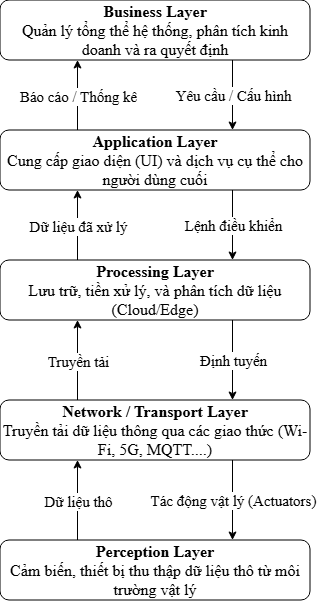
\includegraphics[width=0.4\linewidth]{graphics/LayeredArchitecture.drawio.png}
    \caption{Layered Architecture}
    \label{fig:layered_architecture}
\end{figure}

\subsubsection{Phân tích sự đánh đổi}
Ưu điểm lớn nhất là sự đơn giản trong tư duy thiết kế, giúp đội ngũ triển khai cực nhanh ở giai đoạn khởi tạo (Low entry barrier). Tuy nhiên, khi logic nghiệp vụ trở nên phức tạp, hệ thống có xu hướng biến tướng thành cấu trúc "Big Ball of Mud", gây khó khăn hệ trọng trong việc bảo trì và đọc hiểu mã nguồn. 

Mặc dù các thành phần trong cùng một lớp có tính đóng gói tốt, nhưng giữa các lớp lại tồn tại sự phụ thuộc chặt chẽ. Đặc biệt trong hệ sinh thái IoT, việc thay đổi một giao thức cảm biến mới thường gây ra "hiệu ứng vết dầu loang", buộc kỹ sư phải điều chỉnh mã nguồn đồng loạt trên nhiều tầng khác nhau.

Hạn chế về tính linh hoạt trong việc điều phối tài nguyên. Do các lớp liên kết theo chuỗi, khi tầng thu nhận dữ liệu bị quá tải, hệ thống buộc phải mở rộng toàn bộ ứng dụng thay vì chỉ tập trung vào thành phần đang bị bottleneck.

Kiến trúc này tối ưu cho các nhóm phát triển tinh gọn ($1-3$ người). Ngược lại, với các dự án quy mô lớn, việc phát triển song song thường dẫn đến xung đột luồng công việc và làm chậm tốc độ phân phối tính năng.

Bảng \ref{tab:layered-tradeoffs} dưới đây đúc kết các ưu điểm và hạn chế cốt lõi của mô hình Layered Architecture nhằm cung cấp cái nhìn tổng quan về khả năng vận hành của hệ thống.

\begin{table}[H]
\centering
\caption{Trade-off của Layered Architecture trong IoT}
\label{tab:layered-tradeoffs}
\begin{tabular}{|p{3.5cm}|p{5.5cm}|p{5.5cm}|}
\hline
\textbf{Tiêu chí} & \textbf{Ưu điểm} & \textbf{Nhược điểm} \\ \hline
\textbf{Tư duy thiết kế} & Đơn giản, Low entry barrier, giúp đội ngũ triển khai cực nhanh ở giai đoạn khởi tạo. & Dễ biến tướng thành "Big Ball of Mud" khi logic phức tạp, gây khó khăn lớn cho việc bảo trì và đọc hiểu. \\ \hline
\textbf{Coupling} & Các thành phần trong cùng một lớp có tính đóng gói rất tốt. & Phụ thuộc chặt chẽ giữa các lớp. Thay đổi ở một tầng (như giao thức cảm biến) dễ gây "hiệu ứng vết dầu loang". \\ \hline
\textbf{Điều phối tài nguyên} & Hỗ trợ tốt cho giai đoạn tập trung hiện thực hóa tính năng mà không bị quá tải bởi thiết lập hạ tầng. & Kém linh hoạt, phải mở rộng toàn bộ ứng dụng thay vì chỉ tập trung vào tầng đang bị quá tải (bottleneck). \\ \hline
\textbf{Hiệu năng \& Quy mô} & Tối ưu cho dự án PoC, Prototype, hệ thống nội bộ quy mô nhỏ (dưới 100 thiết bị). & Bị bottleneck khi vượt ngưỡng 1000 thiết bị. Không đáp ứng được Latency khắt khe dưới 100ms. \\ \hline
\textbf{Tổ chức đội ngũ} & Rất phù hợp và tối ưu cho các nhóm phát triển tinh gọn (1-3 người). & Dễ gây xung đột luồng công việc và làm chậm tốc độ phân phối tính năng khi phát triển song song ở dự án lớn. \\ \hline
\end{tabular}
\end{table}

\subsubsection{Ngữ cảnh áp dụng và Ngưỡng tới hạn}
Layered Architecture phát huy tối đa lợi thế trong các kịch bản ưu tiên tính tinh gọn như các dự án Proof of Concept (PoC), phiên bản thử nghiệm (Prototype), hoặc các hệ thống IoT nội bộ với quy mô quản lý dưới $100$ thiết bị. Ở giai đoạn này, cấu trúc phân lớp giúp đội ngũ tập trung vào việc hiện thực hóa tính năng mà không bị quá tải bởi các thiết lập hạ tầng phức tạp.

Tuy nhiên, kiến trúc này bắt đầu bộc lộ những hạn chế hệ trọng khi hệ thống tiến dần đến các ngưỡng vật lý và logic sau. Cụ thể, khi quy mô số lượng thiết bị vượt ngưỡng $1000$ node, khối lượng dữ liệu khổng lồ đi xuyên qua các lớp trung gian sẽ tạo ra bottleneck, khiến chi phí tài nguyên và công sức quản trị tăng theo hàm mũ. Bên cạnh đó, do đặc thù dữ liệu phải tuần tự đi qua từng tầng, kiến trúc này không thể đáp ứng các yêu cầu khắt khe về Latency dưới $100ms$ - một chỉ số sinh tử trong các ứng dụng IoT công nghiệp hoặc điều khiển tự động.

\subsubsection{Summary}
Layered Architecture đóng vai trò là giải pháp nền tảng giúp tối ưu hóa thời gian đưa sản phẩm ra thị trường trong các kịch bản có nguồn lực hạn chế và yêu cầu nghiệp vụ đơn giản. Tuy nhiên, do ràng buộc bởi Tight coupling và cơ chế xử lý tuần tự qua nhiều tầng, mô hình này bộc lộ các hạn chế về hiệu năng và quản trị khi hệ thống dịch chuyển sang quy mô lớn. Cụ thể, kiến trúc này gặp khó khăn trong việc mở rộng riêng lẻ các thành phần có tải cao. Ngoài ra, độ trễ tích lũy qua các lớp gây cản trở các tác vụ phản hồi nhanh trong IoT.